\subsubsection{Example Two}
The second program illustrates the preemption by using an 
immediate weak \verb$abort$ statement. 
Figure~\ref{fig:forec_semantics:program2} presents
the ForeC program and Figure~\ref{fig:forec_semantics:program2_cfg}
illustrates the program's control-flow. In 
Figure~\ref{fig:forec_semantics:program2_cfg}, the
pair of decorated diamonds represents the scope of the 
\verb$abort$ body.

In the program's first tick, the \verb$main$ thread
reaches the immediate and weak \verb$abort$ and immediately
evaluates the preemption condition \verb$(x==1)$. The
condition evaluates to \emph{true} and the preemption is 
triggered. Since the \verb$abort$ is weak, the preemption
is taken only when execution reaches the \verb$pause$, after
the variable \verb$x$ has been incremented. The 
\verb$abort$ terminates and, as a result, the \verb$main$
thread terminates. The first tick ends.

\begin{figure}
	\centering
	
	\hfill
	\begin{minipage}{0.43\columnwidth}
		\subfloat[ForeC program.] {
			\lstinputlisting[style=full]{./code/forec/illustration/program2.forec}
			\label{fig:forec_semantics:program2}
		}

		\subfloat[Translated kernel program.] {
			\lstinputlisting[style=full]{./code/forec/illustration/program2_kernel.forec}
			\label{fig:forec_semantics:program2_kernel}
		}
	\end{minipage}
	\hspace{0.5cm}
	\begin{minipage}{0.28\columnwidth}
		\subfloat[Control-flow graph.] {
			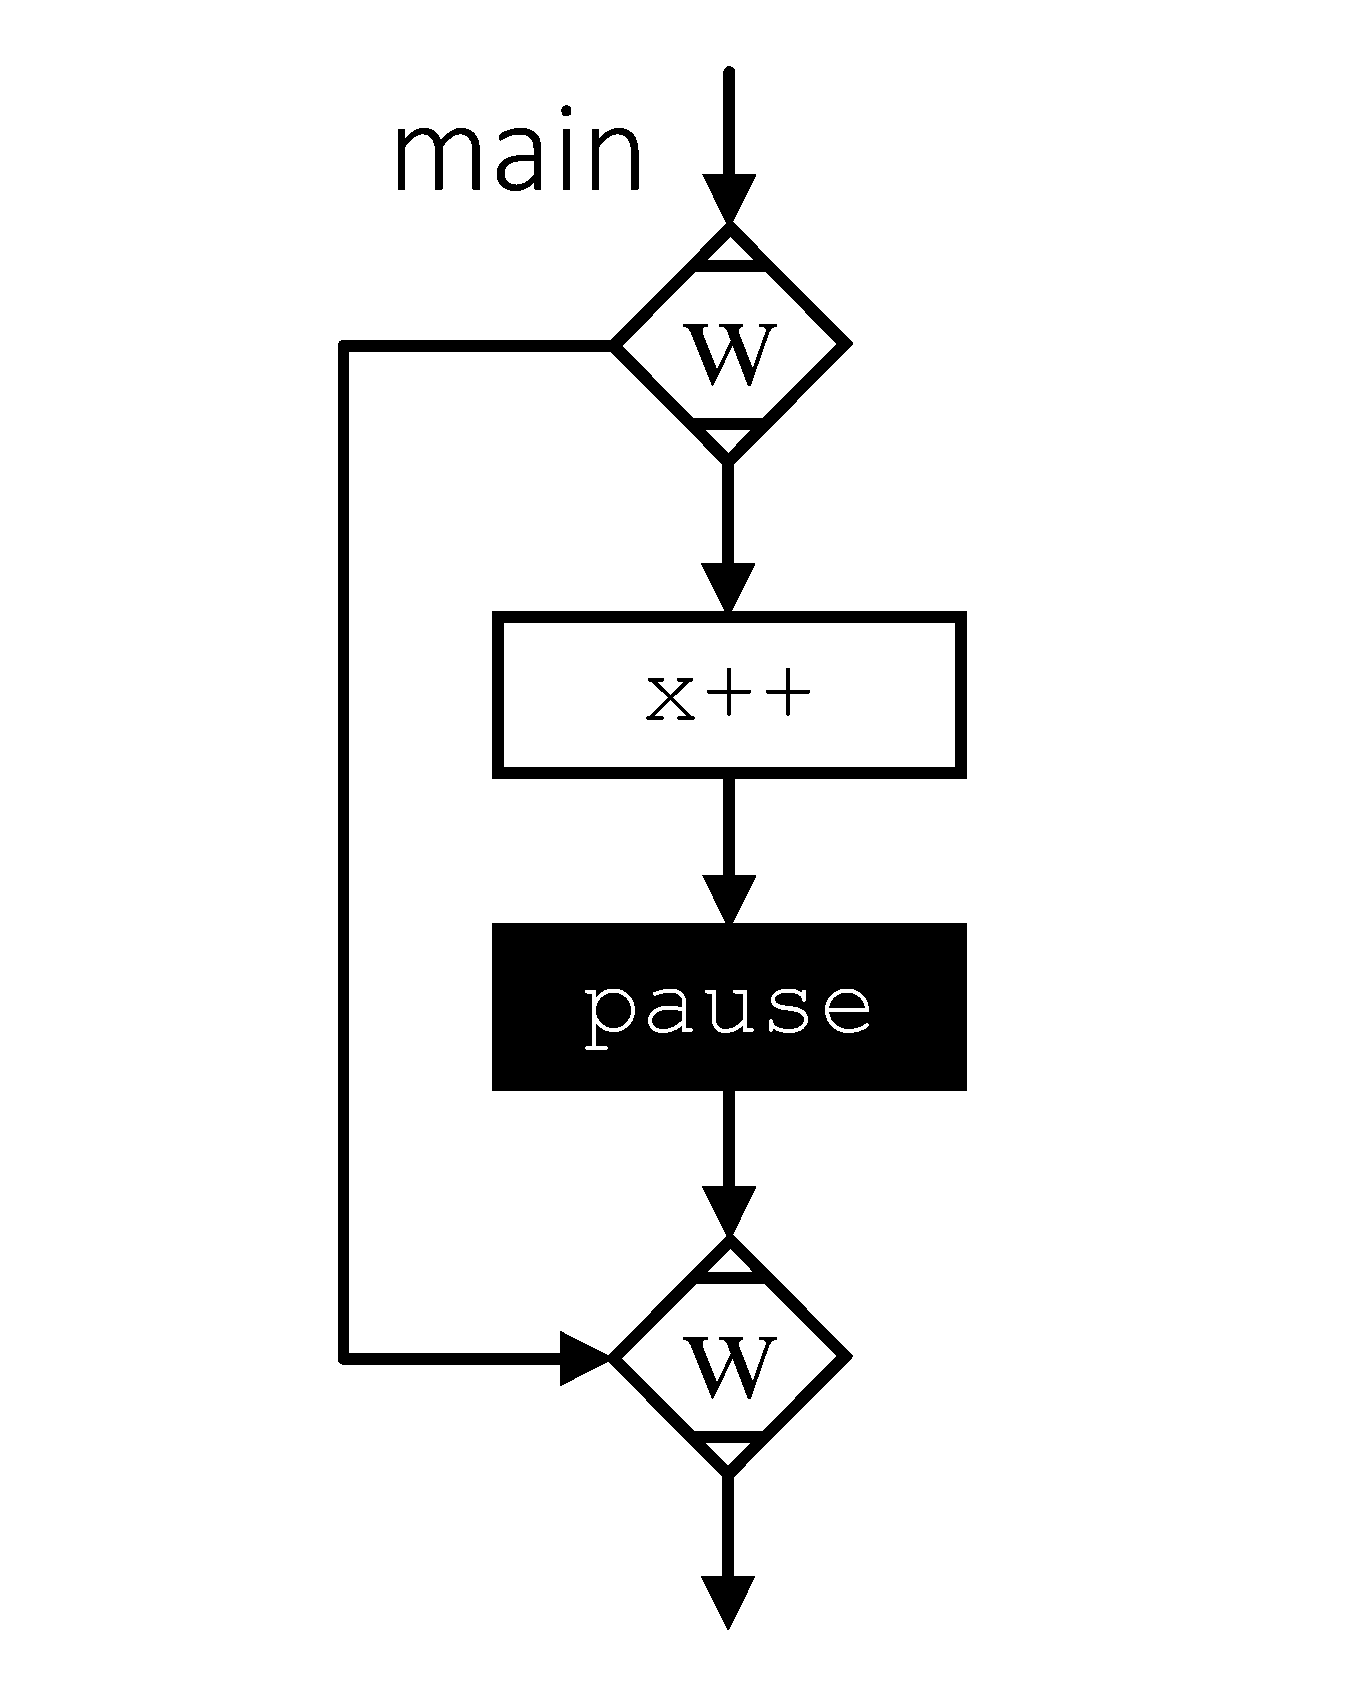
\includegraphics[width=\columnwidth]{program2_cfg}
			\label{fig:forec_semantics:program2_cfg}
		}
	\end{minipage}
	\hspace{1.5cm}

	\caption{Illustrative example two.}
\end{figure}

Before we apply the rewrite rules to the program, 
it is structurally translated into 
Figure~\ref{fig:forec_semantics:program2_kernel} 
(see the start of Section~\ref{sec:forec_semantics}).
The \verb$copy$ kernel statement is not inserted into
the program because no shared variables are used.
Note that the semantic functions $\GetShared($\verb$main$$)$ 
and $\GetShared(\Global)$ all return $\emptyset$.
The program's environment \Environment{}, preemption statuses \Abort{},
and their derivatives are defined in Figure~\ref{figure:forec_program_3}.
\newline

\begin{figure}
	\centering
	$$\begin{array}{l l l l l l}
		\Environment		&=& \left \lbrace
									\Global \to \lbrace x \to (1, \texttt{pvt}) \rbrace
								\right \rbrace	& \qquad 
		\Abort				&=& \lbrace a1 \rbrace			\\
		\Environment^1		&=& \left \lbrace
									\Global \to \lbrace x \to (2, \texttt{pvt}) \rbrace
								\right \rbrace	& \qquad 
		\Abort^1			&=& \lbrace a1 \to 1 \rbrace	\\
		& & & \qquad 
		\Abort^2			&=& \lbrace a1 \to 0 \rbrace
	\end{array}$$
	
	\caption{Initial program state and its derivatives.}
	\label{figure:forec_program_3}
\end{figure}

\noindent
\textbf{Step 1:} Start the tick by applying the
(\ref{forec:seq-right}) and (\ref{forec:status}) rules. Note
that the \verb$abort$'s preemption is triggered because the
condition \verb$x==1$ evaluates to $1$.
\begin{prooftree}
			\AxiomC{}
		\LeftLabel{(\ref{forec:status})}
		\UnaryInfC{$\langle \Environment, \Abort \rangle ~ \texttt{main: status(a1,x==1)}
						\xrightarrow[~~\Input~~]{0} 
					\langle \Environment, \Abort^1 \rangle ~ \texttt{main:}$}
	\LeftLabel{(\ref{forec:seq-right})}
	\UnaryInfC{$\begin{array}{l}
					\langle \Environment, \Abort \rangle ~ \texttt{main:status(a1,x==1);}		\\
					\texttt{weak~abort(a1,\{x++;pause;\})}
				\end{array}
					\xrightarrow[~~\Input~~]{\bot} 
				\begin{array}{l}
					\langle \Environment, \Abort^1 \rangle ~ \texttt{main:weak~abort}		\\
					\texttt{(a1,\{x++;pause;\})}
				\end{array}$}
\end{prooftree}

\noindent
\textbf{Step 2:}
Apply the (\ref{forec:abort-4}), (\ref{forec:seq-right}), and (\ref{forec:assign-private}) rules.
\begin{prooftree}
				\AxiomC{$x \notin \emptyset$}
			\LeftLabel{(\ref{forec:assign-private})}
			\UnaryInfC{$\langle \Environment, \Abort^1 \rangle ~ \texttt{main:x++}
							\xrightarrow[~~\Input~~]{0} 
						\langle \Environment^1, \Abort^1 \rangle ~ \texttt{main:}$}
		\LeftLabel{(\ref{forec:seq-right})}
		\UnaryInfC{$\langle \Environment, \Abort^1 \rangle ~ \texttt{main:x++;pause}
						\xrightarrow[~~\Input~~]{\bot} 
					\langle \Environment^1, \Abort^1 \rangle ~ \texttt{main:pause}$}
	\LeftLabel{(\ref{forec:abort-4})}\RightLabel{$(\Abort^1[a1] \neq 0)$}
	\UnaryInfC{$\begin{array}{l}
					\langle \Environment, \Abort^1 \rangle ~ \texttt{main:weak~abort}		\\
					\texttt{(a1,\{x++;pause;\})}
				\end{array}
					\xrightarrow[~~\Input~~]{\bot} 
				\begin{array}{l}
					\langle \Environment^1, \Abort^1 \rangle ~ \texttt{main:weak~abort}		\\
					\texttt{(a1,\{pause;\})}
				\end{array}$}
\end{prooftree}

\noindent
\textbf{Step 3:}
Apply the (\ref{forec:abort-5}) and (\ref{forec:pause}) 
rules. Note that the preemption is taken because the \verb$abort$'s
body has reached a \verb$pause$.
\begin{prooftree}
			\AxiomC{}
		\LeftLabel{(\ref{forec:pause}) }
		\UnaryInfC{$\langle \Environment^1, \Abort^1 \rangle ~ \texttt{main:pause}
						\xrightarrow[~~\Input~~]{1} 
					\langle \Environment^1, \Abort^1 \rangle ~ \texttt{main:copy}$}
	\LeftLabel{(\ref{forec:abort-5})}\RightLabel{$(\Abort^1[a1] \neq 0)$}
	\UnaryInfC{$\langle \Environment^1, \Abort^1 \rangle ~ \texttt{main:weak~abort(a1,\{pause;\})}
					\xrightarrow[~~\Input~~]{\bot} 
				\langle \Environment^1, \Abort^1 \rangle ~ \texttt{main:copy}$}
\end{prooftree}

\noindent
\textbf{Step 4:}
Apply the (\ref{forec:tick}) and (\ref{forec:copy}) 
rules. The preemption statuses in $\Abort^1$ are
updated to be~$\Abort^2$.
\textbf{The tick ends and the program terminates.}
\begin{prooftree}
			\AxiomC{}
		\LeftLabel{(\ref{forec:copy})}
		\UnaryInfC{$\langle \Environment^1, \Abort^1 \rangle ~ \texttt{main:copy}
						\xrightarrow[~~\Input~~]{0} 
					\langle \Environment^1, \Abort^1 \rangle ~ \texttt{main:}$}
	\LeftLabel{(\ref{forec:tick})}
	\UnaryInfC{$\langle \Environment^1, \Abort^1 \rangle ~ \texttt{main:copy}
					\xrightarrow[~~\Input~~]{0} 
				\langle \Environment^1, \Abort^2 \rangle ~ \texttt{main:}$}
\end{prooftree}
